\subsection{Como o Flux funciona?}

Esta seção irá esclarecer como o Flux denomina cada parte do BPM e como é feita sua criação para implementação dentro do mesmo. Essas definições serão importantes para melhor leitura das implementações feitas no Flux para resolverem os problemas falados.

\subsubsection{Atributos, Atividades e Instâncias}

Os atributos de uma atividade definem as informações que poderão ser acrescentadas a uma atividade, isto é, os atributos definem quais dados poderão ser adicionados a cada atividade, definindo também seu tipo (número, texto...), obrigatoriedade, correlação com outros atributos, e um conjunto de atributos em um passo específico de um workflow forma uma atividade.

Uma atividade em um workflow define um passo no BPM modelado. Em um workflow, podem existir qualquer número de atividades, sendo uma atividade inicial para iniciar o BPM, seguido de atividades dependentes das atividades anteriores em um formato de árvore na definição computacional, como podemos ver na figura~\ref{fig:bpmn_diagram}

\begin{figure}
    \centering
    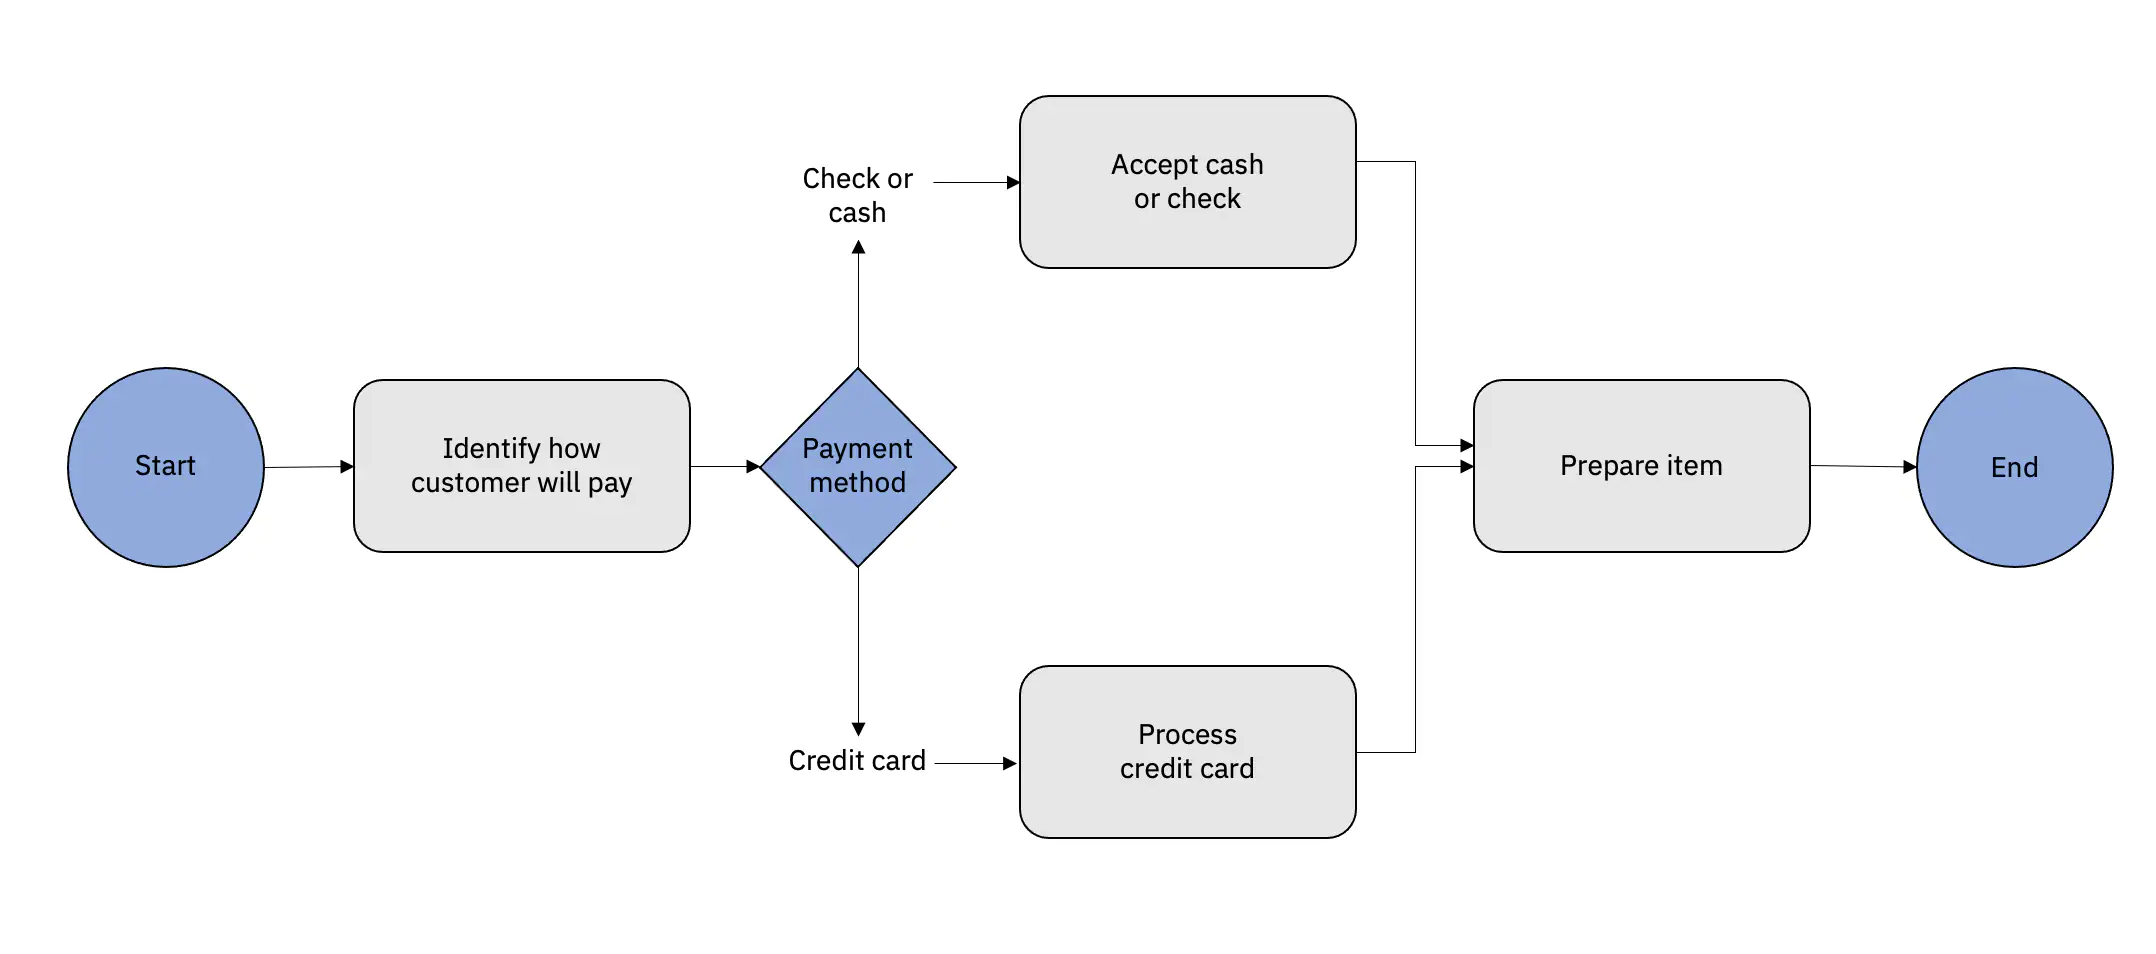
\includegraphics[width=0.7\textwidth]{imgs/BPM/bpmn_diagram.png}
    \caption{Exemplo de um diagrama projetado utilizando BPMN. Imagem da IBM~\cite{TheIBM}}
    \label{fig:bpmn_diagram}
\end{figure}

Um conjunto de atividades formam um workflow modelado dentro do software. Esse conjunto de atividades deve ser executado uma ou mais vezes, definindo ações que podem ser executadas para executar um processo. Neste caso, necessitamos que estas atividades estejam separadas para cara execução, para que o dados possam ser registrados para apenas aquela execução.

Para isso, o Flux utiliza de instâncias, que nada mais é que uma separação entre as diferentes execuções de um workflow. Cada instância é criada quando executamos a primeira atividade do workflow selecionado, definindo o início de um novo processo a ser executado.

Um workflow pode ter uma ou mais instâncias, sendo a execução delas o ponto principal do Flux.
Cada workflow pode ser criado através do editor de workflows que existe dentro do próprio Flux, onde podem ser construídos e editados para seguirem um BPM modelado para a organização que irá utilizá-lo.

O editor de workflows funciona de maneira intuitiva para o usuário, sem a necessidade de utilizar nenhuma linguagem de programação, apenas arrastar atributos para atividades criadas e criar atividades seguindo um modelo construído (Podemos ver um exemplo do workflow CENTRARE na figura~\ref{fig:editor_centrare}).

Atividades podem ser filhas de outra atividade, ou seja, elas dependem da execução da atividade pai para que elas possam ser executadas, ou podem ser irmãs de outras atividades, que significa que a sua execução não interfere na execução da atividade irmã, mas que as duas só ficam disponíveis quando a atividade pai delas for executada. Podemos visualizar exemplos de workflow na figura~\ref{fig:estrutura_workflow}.

\begin{figure}
    \centering
    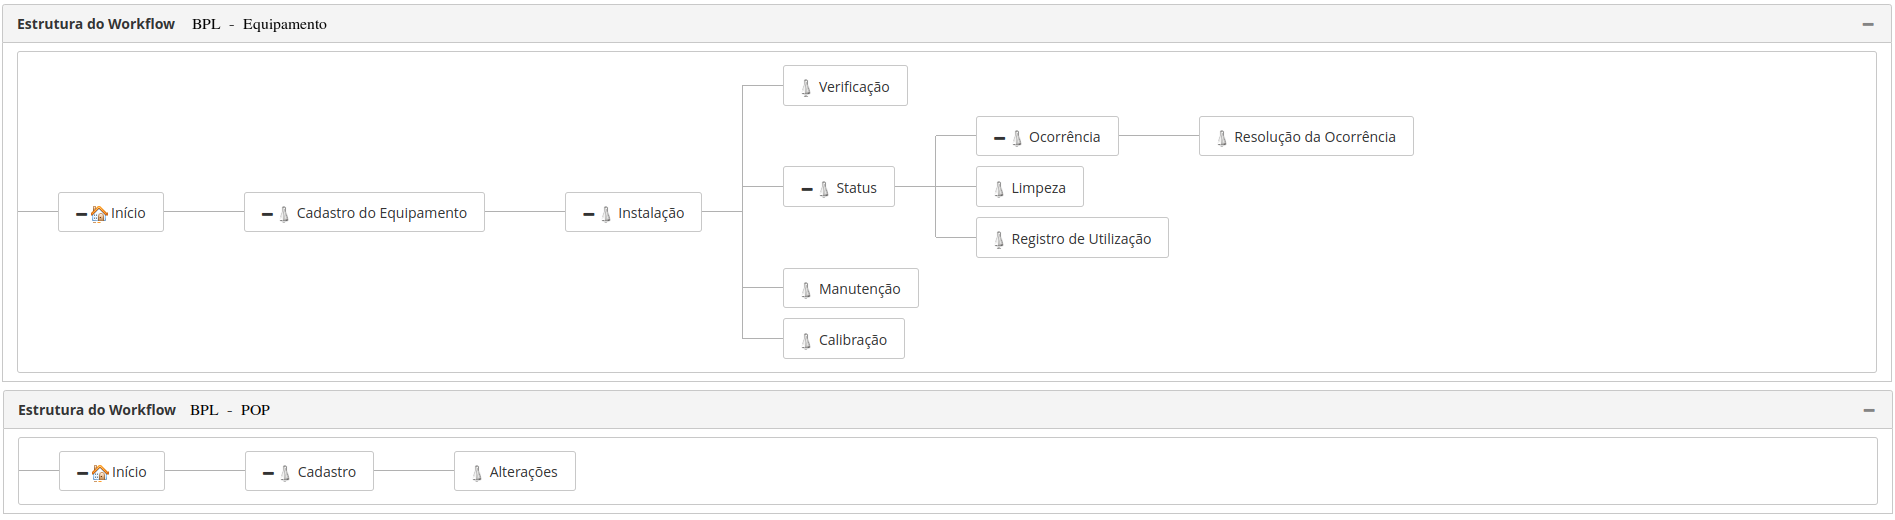
\includegraphics[width=1\textwidth]{imgs/BPL/estrutura.png}
    \caption{Estrutura de dois workflows: BPL - POP e BPL Equipamentos. A atividade inicial destes workflows são as atividades "Cadastro" e "Cadastro do equipamento", respectivamente.}
    \label{fig:estrutura_workflow}
\end{figure}

\begin{figure}
    \centering
    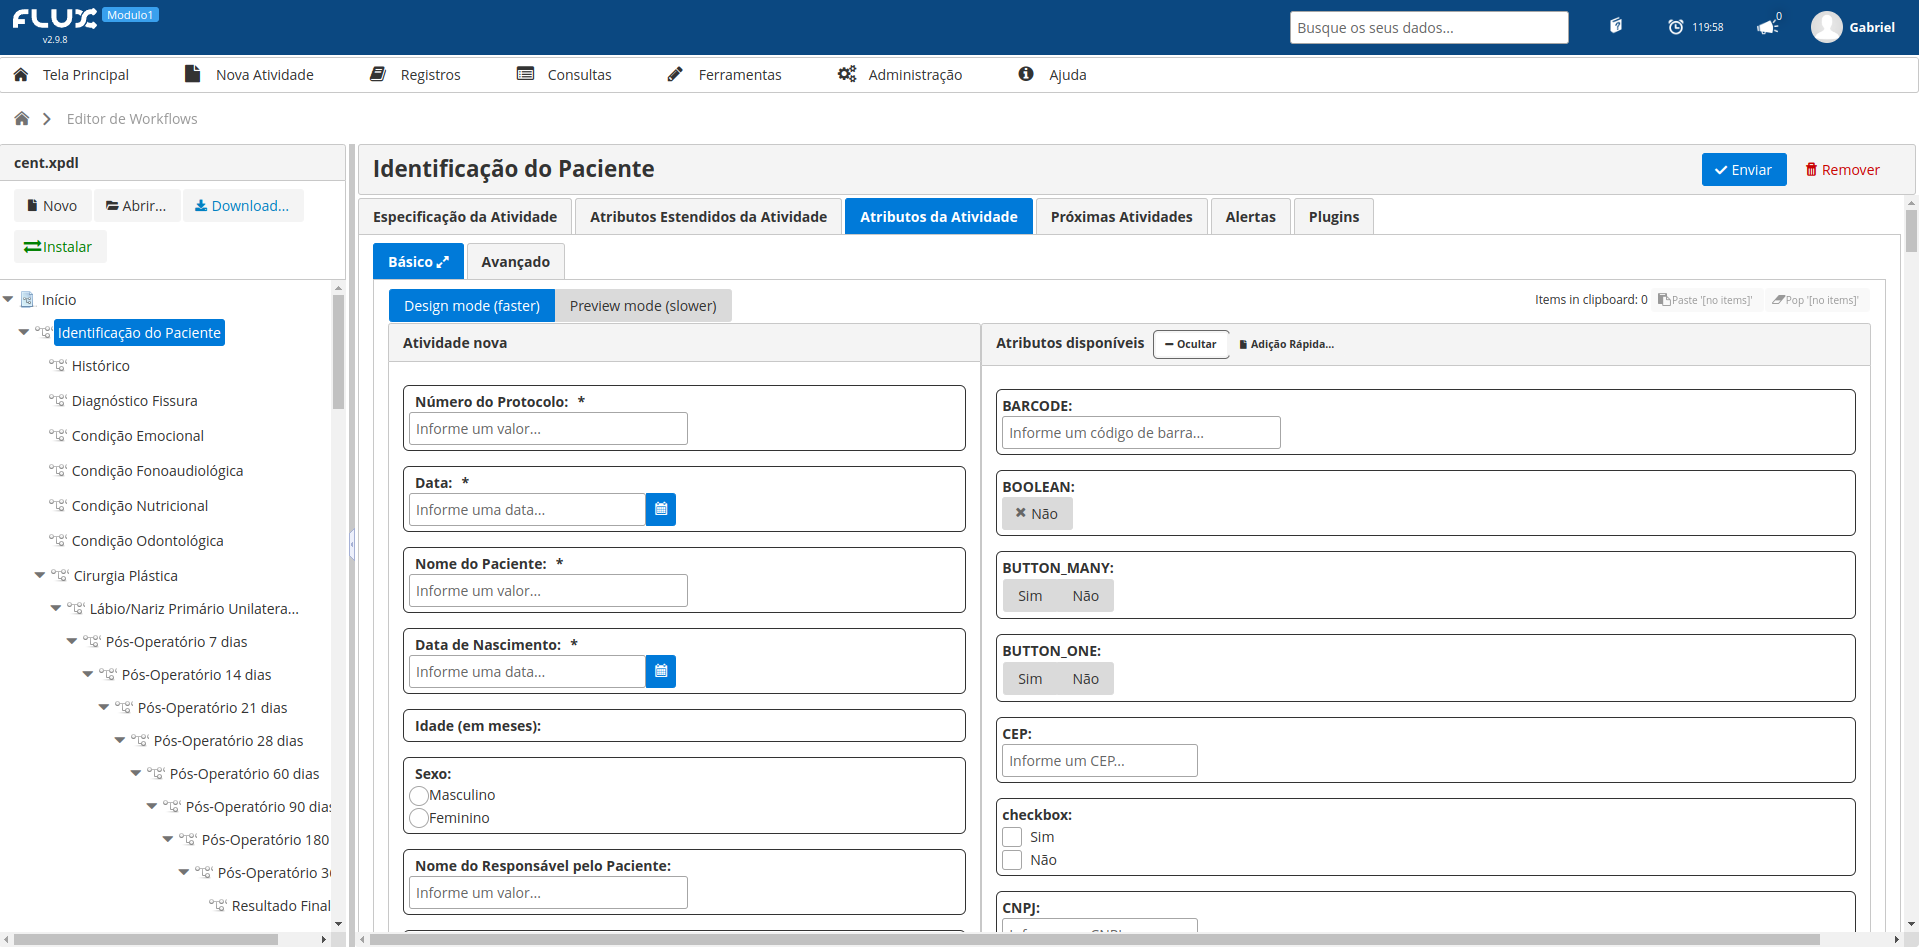
\includegraphics[width=1\textwidth]{imgs/Flux/Workflows/Editor/editor_centrare.png}
    \caption{Visualização da primeira atividade do workflow CENTRARE e seus atributos no editor de workflows do LIMS Flux. Podemos ver a árvore de atividades no canto esquerdo da tela, bem como os atributos da atividade na tabela "Atividade nova" e atributos disponíveis para serem adicionados na atividade na tabela "Atributos disponíveis".}
    \label{fig:editor_centrare}
\end{figure}

\subsubsection{Transições} \label{sec:transitions}

No Flux existe o conceito de transições. Uma transição define uma relação de dependência entre duas atividades. Para que exista uma atividade B filha de A, deve-se existir uma transição entre elas. Cada transição demonstra uma relação de dependência entre as atividades filha e as atividades pai (como visto na figura~\ref{fig:transitions})

Também ocorre a existência de transições entre atividades que não são pais e filhas, que nada mais é a criação de uma transição entre elas. Quando isso ocorre, a transição criada dita que existe uma correlação de dependência entre duas atividades sem a necessidade delas estarem na mesma subárvore de um workflow.

Caso exista múltiplas transições de atividades pai para uma filha (por meio deste tipo de transições), a atividade será disponibilizada na execução de qualquer uma das atividades pai da mesma.

\begin{figure}
    \centering

    \begin{subfigure}[b]{0.45\textwidth}
        \centering
        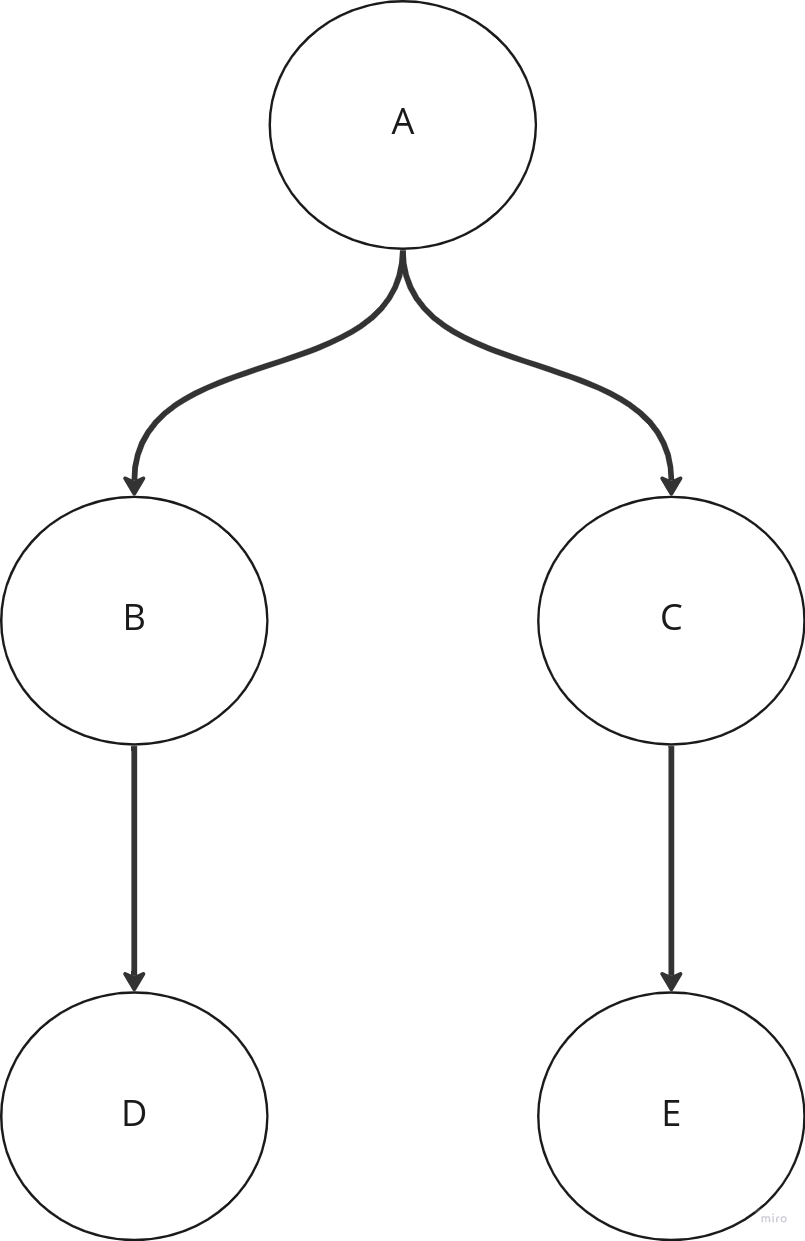
\includegraphics[width=0.6\textwidth]{imgs/Flux/Transicoes/normal.png}
        \caption{Transições entre atividades. Atividade A é a atividade inicial e tem duas atividades filhas: B e C. Delas, temos a atividade D que é filha de B e a atividade E que é filha de C.}
        \label{fig:transition_normal}
    \end{subfigure}
    \hfill
    \begin{subfigure}[b]{0.45\textwidth}
        \centering
        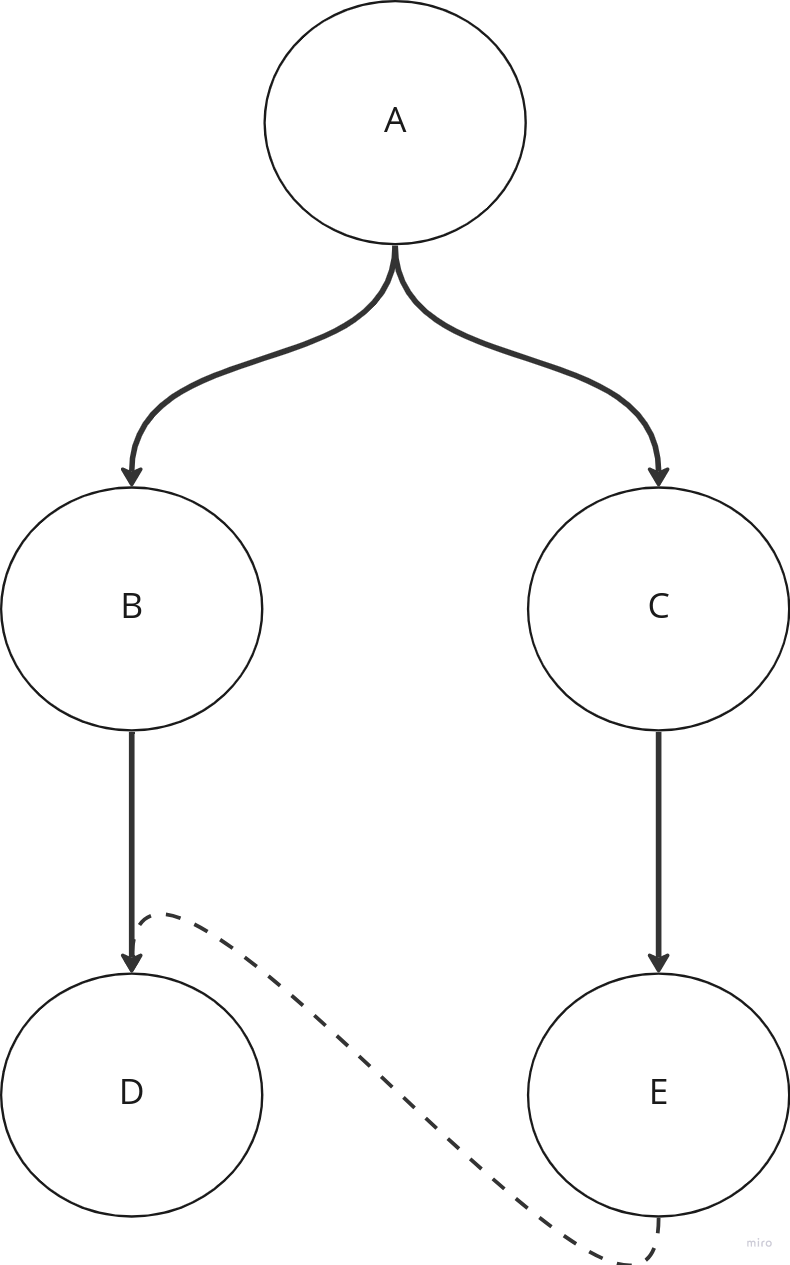
\includegraphics[width=0.6\textwidth]{imgs/Flux/Transicoes/referencia.png}
        \caption{Neste exemplo temos as mesmas transições mostradas em~\ref{fig:transition_normal}, mas com uma transição da atividade E para a atividade D (demonstrada pela seta pontilhada). A atividade D será disponibilizada quando o usuário executar a atividade B OU quando executar a atividade E.}
        \label{fig:transition_ref}
    \end{subfigure}
    \caption{Demonstração de transições entre atividades dentro do Flux. Cada atividade é representada por um circulo e cada seta entre círculos representa uma transição.}
    \label{fig:transitions}
\end{figure}

\subsubsection{Usuários do Flux}

Existem dois tipos de usuários dentro do Flux: Usuários administradores e usuários comuns.

Usuários administradores podem gerenciar todos os quesitos do LIMS para que ele seja moldado para a organização a que pertence. Administradores podem criar workflows dentro do software, configurar permissões de usuários comuns sobre o acesso deles a atividades, instâncias e workflows, além de gerenciar as contas dos próprios usuários comuns.

Os usuários comuns são pessoas que apenas executarão os workflows criados pelos administradores. O usuário comum só poderá visualizar, aprovar, executar, gerar relatórios de atividades que lhe foi dado permissão pelos administradores.

Múltiplos usuários podem executar instâncias diferentes ou até mesmo a mesma instância de um workflow utilizando o Flux. Desta maneira, pode-se integrar múltiplos participantes de um mesmo processo para executarem em paralelo atividades que façam parte do mesmo BPM.

\subsubsection{Grupos de usuários}

O Flux também permite a criação de grupos de usuários. A criação de grupos é feita pelo usuário administrador, que pode gerenciar quais usuários pertencem a que grupos.

Estes grupos criados facilitam a atribuição de permissões em massa para workflows que serão compartilhados com muitos usuários.

Um usuário pode pertencer a um ou mais grupos como demonstrado na figura~\ref{fig:user_edit}.

\begin{figure}
    \centering
    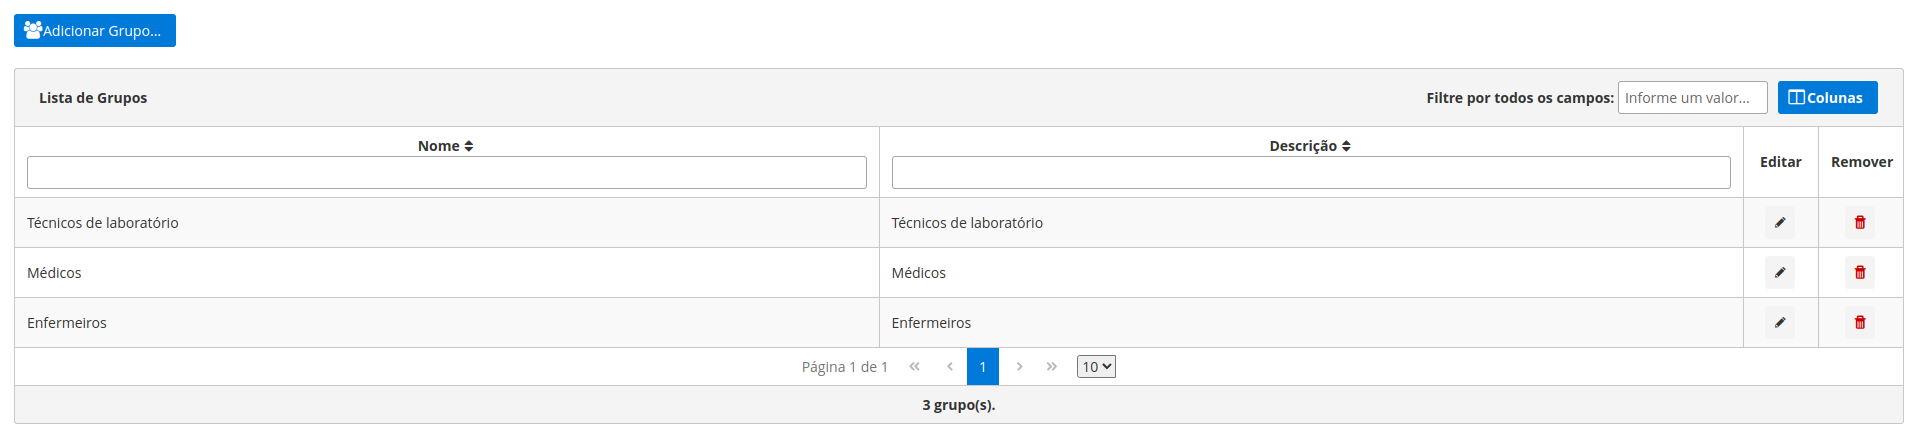
\includegraphics[width=\textwidth]{imgs/Flux/Grupos/listaDeGrupos.png}
    \caption{Lista de grupos criado em um sistema LIMS}
    \label{fig:groups_list}
\end{figure}

\begin{figure}
    \centering
    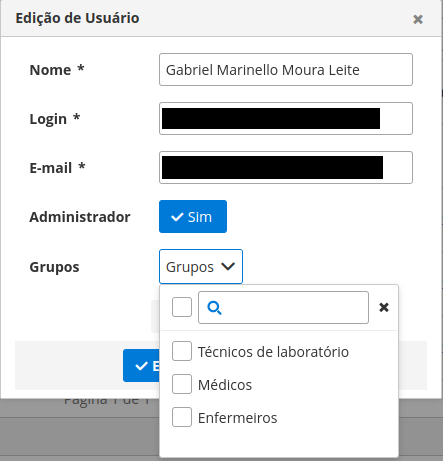
\includegraphics[width=\textwidth, height=7.5cm, keepaspectratio]{imgs/Flux/Usuarios/edicaoUsuario.png}
    \caption{Edição de um usuário. Percebe-se que o usuário pode ser adicionado a um ou mais grupos pela lista de seleção apresentada pela interface no canto inferior da figura.}
    \label{fig:user_edit}
\end{figure}

\subsubsection{Sistema de permissões}

O Flux implementa um sistema de permissões completo, com diferentes níveis de permissão para atividades, instâncias e workflows.
Um usuário administrador do sistema pode gerenciar tais permissões por meio da interface de permissões, que permite a configuração de permissões tanto para usuários individuais quanto para grupos de usuários (demonstrado na figura~\ref{fig:permission_interface}).

Existem 5 níveis de permissão no sistema hoje:

\begin{itemize}
    \item Visualização: Permite ao usuário visualizar a atividade.
    \item Executar: Permite ao usuário inserir dados em uma atividade e executá-la (Gravá-la no banco de dados).
    \item Editar: Permite que o usuário edite dados de uma atividade já executada.
    \item Aprovar: Quando uma atividade for executada, seja pelo usuário com permissão ou por outro usuário, permite que o usuário aprove os dados da atividade. Atividades filhas só ficarão disponíveis com esta aprovação.
    \item Gerar Relatório: Permite que o usuário imprima um relatório da atividade.
\end{itemize}

Cada uma dessas permissões podem ser atribuídas separadamente para cada usuário e/ou grupo de usuários, para cada atividade de um workflow (como demonstrado na figura~\ref{fig:permission_activity_interface}).

Caso um usuário pertença a um grupo de usuários que detêm um conjunto de permissões, este usuário irá receber todas as permissões atribuídas àquele grupo. Com isso, há uma maior facilidade para atribuição de permissões para múltiplos usuários ao mesmo tempo com a criação de grupos diferentes para cada setor da organização, já que pode existir um número grande de atividades no workflow modelado.

\begin{figure}
    \centering
    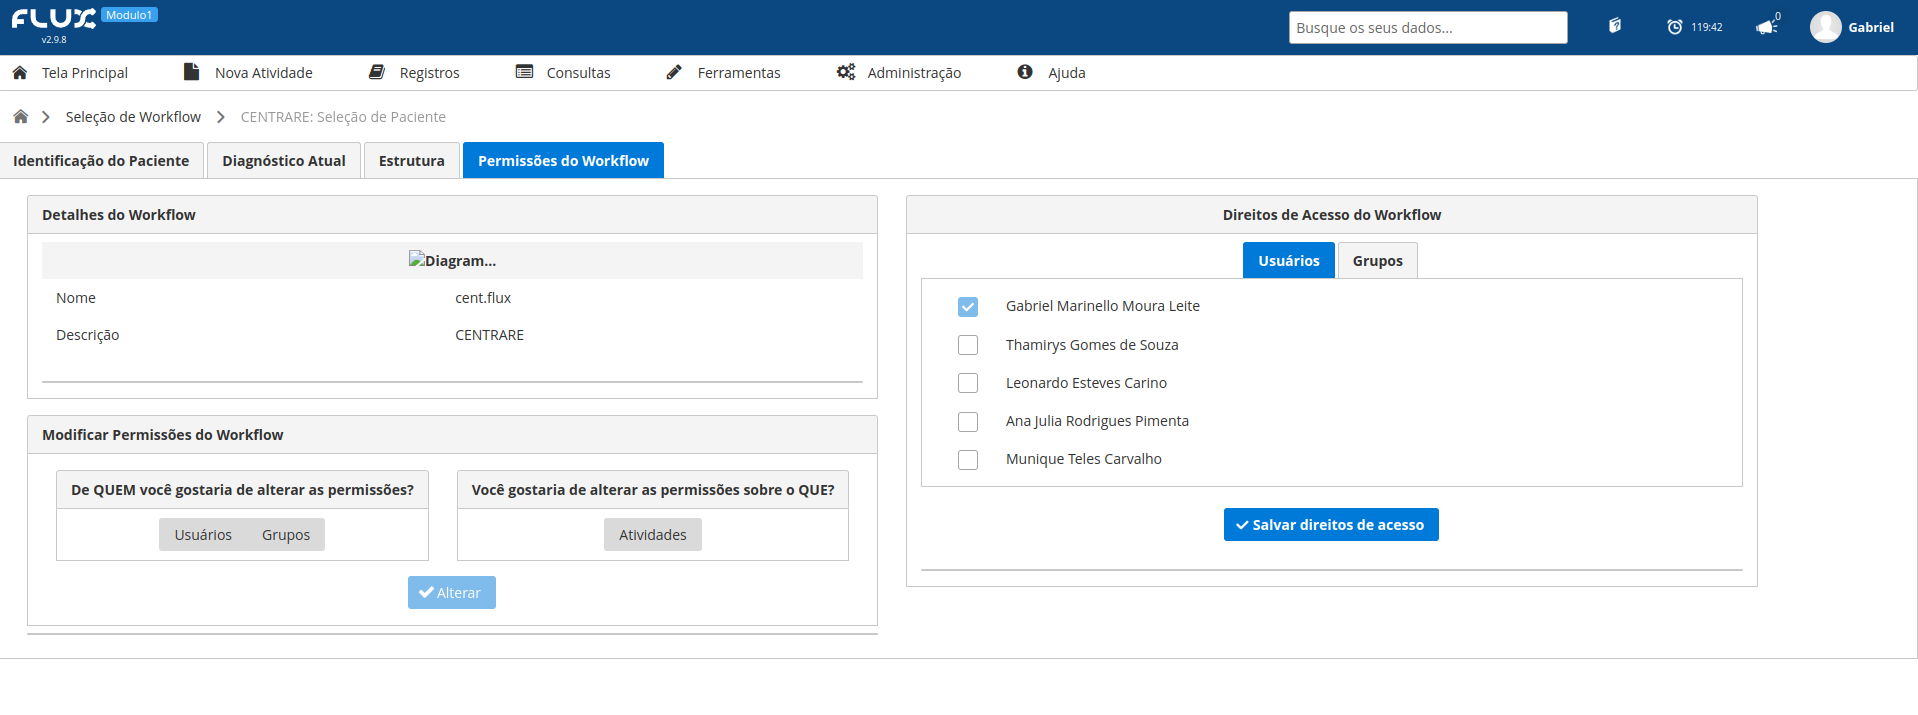
\includegraphics[width=\textwidth]{imgs/Flux/Permissoes/telaPermissoesCENTRARE.png}
    \caption{Interface para alteração de permissões de um workflow (neste caso, do workflow CENTRARE). Caso um usuário não tenha nenhuma permissão em um workflow, o workflow não aparece na interface deste usuário (Usuários desmarcados no canto direto da tela).}
    \label{fig:permission_interface}
\end{figure}

\begin{figure}
    \centering
    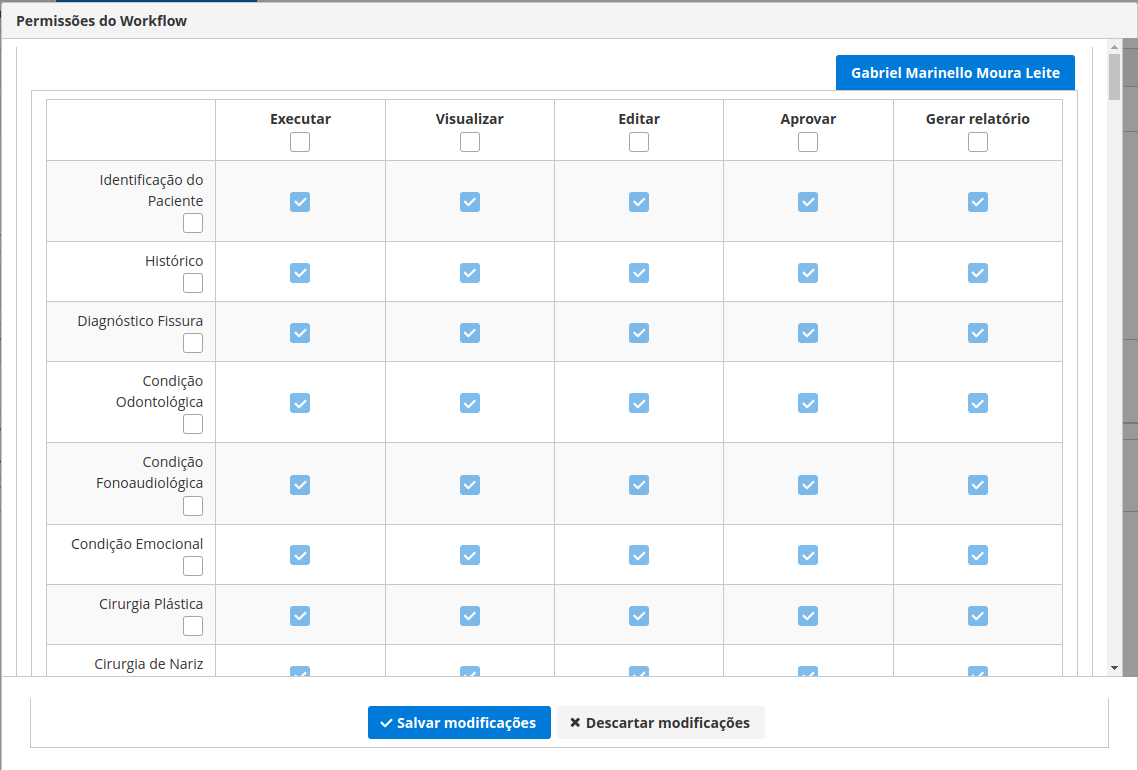
\includegraphics[width=\textwidth]{imgs/Flux/Permissoes/telaPermissoeAstividadesCENTRARE.png}
    \caption{Tela para adição de permissões em atividades do workflow CENTRARE. O usuário administrador pode atribuir permissões diferentes para cada atividade, para cada usuário ou grupo de usuários.}
    \label{fig:permission_activity_interface}
\end{figure}